\subsection{Campaña integrada A0--FULL: cadena de coalición física}
\label{sec:campana-integrada-certificados}

SP1--SP8 aíslan mecanismos con plantas distintas. A0--FULL cierra esa brecha mediante
seis tratamientos acumulativos sobre un único simulador. A0 calcula una utilidad por
robot y aplica un umbral global; no es un juego formal. A1 añade cuórum entero global;
A2, capacidad efectiva; A3, complementariedad de contactos mediante una búsqueda global
acotada; A4, reserva dinámica y HOCBF; y FULL incorpora mensajes con retardo, pérdida y
memoria expirable, además de un selector global de reemplazo usado como proxy.

El protocolo correctivo v1.1 se congeló después de un \emph{dry-run} de 24 casos y de
V1--V3, antes de abrir semillas nuevas. Fijó 100 mundos por familia y ejecutó los seis
tratamientos sobre cada mundo: $4\times100\times6=2.400$ filas únicas, sin parada
opcional ni errores numéricos. Los veinte estimandos, pruebas, semillas de \emph{bootstrap}
y la corrección de Holm se fijaron en el contrato de hipótesis. La ejecución usó cuatro
procesos CPU, sin GPU, CoppeliaSim ni entrenamiento nuevo. La campaña adaptativa v1 queda
supersedida y no se mezcla con estas estimaciones.

\subsubsection{Semántica y resultados}

La planta y las comprobaciones se derivan en la
Sección~\ref{sec:nucleo-matematico-coalicion}. \texttt{accepted\_by\_stage} acredita
solo lo que el escalón conoce; \texttt{final\_physical\_success} exige además llegada,
ausencia de colisión y recuperación; \texttt{physical\_false\_positive} identifica una
aceptación que falla al ejecutar. Una asignación que colisiona no se convierte en éxito
por haber resuelto el problema estático.

\begin{figure}[H]
  \centering
  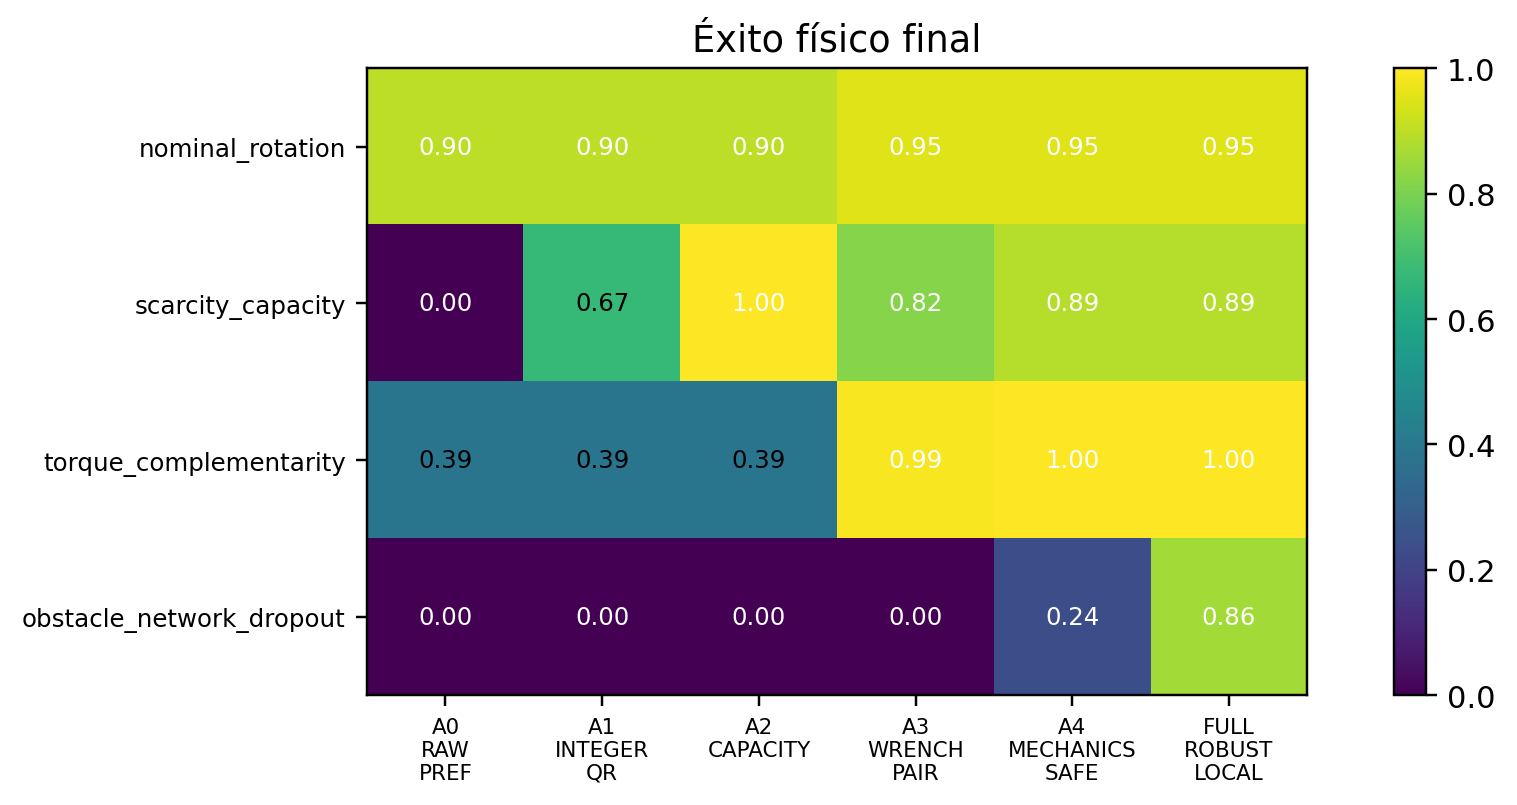
\includegraphics[width=0.86\textwidth]{figures/fig-certificate-success-heatmap.png}
  \caption{Éxito físico por familia y prefijo acumulativo en 100 mundos por familia. La figura muestra frecuencias dentro del generador, no prevalencias industriales.}
  \viuownsource
  \label{fig:certificate-success-heatmap}
\end{figure}

\begin{table}[H]
\centering
\footnotesize
\begin{tabularx}{\textwidth}{@{}Xrrrr@{}}
\toprule
Familia & $n$ & Éxito FULL & Falso positivo & Mensajes medios \\
\midrule
Nominal con rotación & 100 & $1{,}00$ & $0{,}00$ & $442{,}36$ \\
Escasez de capacidad & 100 & $0{,}92$ & $0{,}08$ & $503{,}38$ \\
Complementariedad de momento & 100 & $1{,}00$ & $0{,}00$ & $431{,}79$ \\
Obstáculo, red y \emph{dropout} & 100 & $0{,}89$ & $0{,}11$ & $631{,}84$ \\
\bottomrule
\end{tabularx}
\caption{Desempeño del escalón FULL en la campaña integrada de tamaño fijo.}
\label{tab:integrated-full-results}
\end{table}

En escasez, A1 mejoró a A0 en $0{,}56$ (IC95\% $[0{,}46,0{,}65]$;
$p_{\rm Holm}=5{,}00\times10^{-16}$) y A2 añadió $0{,}44$
($[0{,}34,0{,}54]$; $p_{\rm Holm}=1{,}93\times10^{-12}$). A3 redujo después el
éxito en $0{,}16$ ($[-0{,}24,-0{,}09]$;
$p_{\rm Holm}=4{,}58\times10^{-4}$): retiró un robot estáticamente redundante cuya
fuerza aumentaba la autoridad de seguimiento. A4 recuperó $0{,}08$, pero el contraste
no sobrevivió Holm ($p_{\rm Holm}=0{,}109$).

En complementariedad de momento, A3 mejoró a A2 en $0{,}63$ (IC95\%
$[0{,}54,0{,}72]$; $p_{\rm Holm}=4{,}12\times10^{-18}$). Dos contactos
complementarios generaron un momento que no se deduce de la capacidad escalar. En la
familia de obstáculo y \emph{dropout}, A4 añadió $0{,}22$ ($[0{,}14,0{,}30]$) y
FULL añadió $0{,}67$ ($[0{,}58,0{,}76]$); ambos efectos permanecieron tras Holm. El
último estimando corresponde al paquete memoria--comunicación--reemplazo y no identifica
por separado sus componentes. En nominal, A3--A2 fue $0{,}07$ con IC95\%
$[0{,}02,0{,}1203]$, pero no superó la familia Holm ($p_{\rm Holm}=0{,}203$).

\begin{figure}[H]
  \centering
  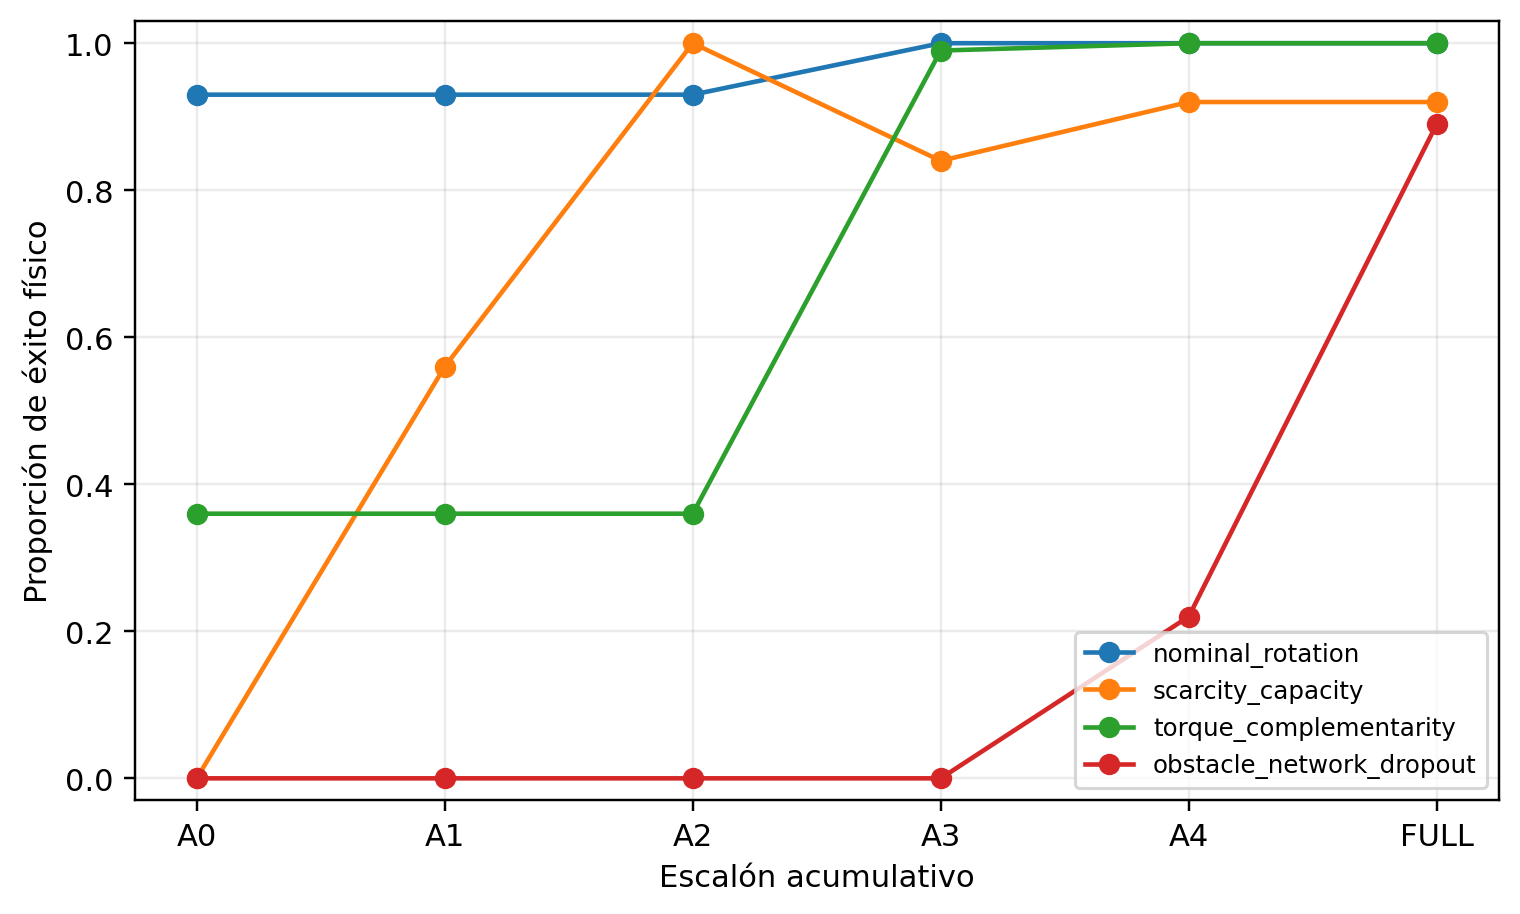
\includegraphics[width=0.72\textwidth]{figures/fig-cumulative-certificate-ladder.png}
  \caption{Evolución del éxito al añadir comprobaciones. La caída A2--A3 en escasez separa factibilidad estática y autoridad dinámica; las barras no implican monotonía.}
  \viuownsource
  \label{fig:cumulative-certificate-ladder}
\end{figure}

\subsubsection{Fallo residual, parámetros y alcance}

FULL alcanzó $0{,}89$--$1{,}00$, pero no domina por construcción. Conserva un 8\% de
falsos positivos en escasez y un 11\% de colisiones en obstáculo. En esta última familia,
75 mundos activaron exactamente un reemplazo y 25 no activaron ninguno; no hubo más de
un reemplazo por evento ni \emph{dropouts} sin recuperar. Los once fallos restantes
aparecen cuando el conjunto de contactos no reproduce la aceleración HOCBF. La seguridad
se decide por el despeje ejecutado, no por la mera salida del filtro. FULL eleva los
mensajes medios a 432--632, frente a 6--8 en A0. Las trayectorias representativas son
post-hoc y no se usaron para seleccionar semillas.

\begin{table}[H]
\centering
\scriptsize
\begin{tabularx}{\textwidth}{@{}p{0.18\textwidth}p{0.23\textwidth}p{0.22\textwidth}X@{}}
\toprule
Parámetro & Valor o dominio evaluado & Mecanismo/endpoint afectado & Sensibilidad y riesgo de inversión \\
\midrule
Residual estático $\rho$ & Umbral $0{,}16$; sin barrido. & Aceptación \emph{wrench} y cambios A2--A3. & No estimada; variar el umbral puede alterar altas/bajas y la caída en escasez. \\
Carga & Masa 18~kg; inercia $5{,}2$~kg\,m$^2$; amortiguación fija. & Autoridad, seguimiento y A3--A4. & No estimada; otra planta puede cambiar éxito y cota ISS. \\
Integración & $\Delta t=0{,}1$~s; horizonte 22~s. & Llegada, timeout y colisión discreta. & No estimada; no autoriza invariancia continua. \\
Seguridad & Radio $0{,}82$~m; $k_1=k_2=2{,}4$; 8 pasadas. & Proyección HOCBF y despeje. & No estimada; una orden SAFE puede ser no realizable tras saturación. \\
Robots & Capacidad $[6,12]$; fuerza $[4{,}5,8{,}5]$~N; salud $[0{,}62,1]$. & Cuórum, capacidad y \emph{wrench} ejecutable. & Variados por mundo, no mediante factorial confirmatorio independiente. \\
Demanda $[F_x,F_y,M_z]$ & Nominal $[11,0{,}4,1{,}8]$; escasez $[13,0{,}8,1{,}6]$; momento $[10,0,\pm5{,}2]$; obstáculo $[12,1,2{,}4]$. & Contrastes por familia. & Solo cuatro regímenes; no define una frontera continua de operación. \\
Red y fallo & Pérdida $0{,}02$/retardo 1 paso; adverso $0{,}22$/3 pasos; baja a 7,5~s. & Memoria, mensajes y FULL--A4. & Efecto conjunto; no identifica pérdida, retardo y reemplazo por separado. \\
Contacto/fricción & Agarre rígido planar; fricción y deslizamiento no modelados. & Transferencia de fuerza y validez física. & Sin intervalo plausible evaluado; puede invertir cualquier conclusión de ejecución. \\
\bottomrule
\end{tabularx}
\caption{Parámetros que condicionan A0--FULL y riesgo de extrapolación. ``No estimada'' significa que la campaña no contiene un diseño de sensibilidad paramétrica.}
\label{tab:parametros-integrados}
\end{table}

No se añadió una sensibilidad post-hoc: habría requerido elegir dimensiones y rangos
después de observar los resultados y no habría reparado el diseño adaptativo original.
La corrección adoptada fue una nueva campaña con semillas frescas, tamaño fijo y contrato
inferencial congelado. Por tanto, \emph{robustez} significa variación dentro de las cuatro
familias ensayadas, no robustez paramétrica general. El reemplazo consulta el conjunto
global de robots ociosos; FULL respalda un proxy de recuperación bajo mensajes degradados,
no un cierre local totalmente distribuido. También se requieren estado inicial seguro,
agarre rígido establecido y autoridad suficiente para realizar el \emph{wrench} SAFE.

El aporte no consiste en una mejora monótona. La cadena localiza qué supuesto falla y
muestra que cerrar una restricción puede degradar otra al retirar margen físico. Esa
interacción entre selección, geometría, dinámica, seguridad e información es el resultado
que las campañas modulares no podían establecer.
